Here we have a use case diagram displaying an actors interaction with our 
system. It shows the functionality available to both the client, and the 
operator. We also have a sequence diagram to augment the use case diagrams.

%\begin{landscape}

\begin{tikzpicture}

%Actor Declaration
\umlactor[x=0,y=8]{Client}

\begin{umlsystem}[x=4,y=0]{System}
%Client Use case Declarations

%Public Key Use Cases
\umlusecase[name=ucPublicKey,x=0,y=4]{Manage Relations}
\umlusecase[name=ucAddAuthorise,x=5,y=3]{Add/Authorise}
\umlusecase[name=ucAddPublicKey,x=10,y=3]{Public Key}
\umlusecase[name=ucQrCode,x=10,y=2]{QR Code}
\umlusecase[name=ucCategorise,x=5,y=4]{Categorise}
\umlusecase[name=ucIgnore,x=5,y=5]{Ignore}

%Account Use Cases
\umlusecase[name=ucAccount,x=0,y=7]{Account Management}
\umlusecase[name=ucCreateClaim,x=5,y=6]{Create/Claim}
\umlusecase[name=ucPDATA,x=5,y=7]{Profile Data}
\umlusecase[name=ucDataAdd,x=10,y=6]{Add Profile Data}
\umlusecase[name=ucDataEditUpdate,x=10,y=7]{Edit/Update}

%Communication Use Cases
\umlusecase[name=ucCommunication,x=0,y=10.5]{Communication}
\umlusecase[name=ucEncrypt,x=5,y=8]{Encrypt}
\umlusecase[name=ucDecrypt,x=2,y=8]{Decrypt}
\umlusecase[name=ucRtChat,x=5,y=9]{Real-Time Chat}
\umlusecase[name=ucPost,x=5,y=10]{Post}
\umlusecase[name=ucPostOwnWall,x=10,y=9]{Own Wall}
\umlusecase[name=ucPostOtherWall,x=10,y=10]{Other's Wall}
\umlusecase[name=ucComment,x=5,y=11]{Comment}
\umlusecase[name=ucLike,x=5,y=12]{Like}
\umlusecase[name=ucUpdateDb,x=5,y=13]{Event}

%Revoke Use Case
\umlusecase[name=ucRevoke,x=0,y=14]{Revoke Private Key}

\end{umlsystem}

%Start of Client's Relations

%Public Key Relations
\umlassoc[name=assClientPublicKey]{Client}{ucPublicKey}
\umlextend[name=extPublicAdd]{ucAddAuthorise}{ucPublicKey}
\umlextend[name=extPublicCategorise]{ucCategorise}{ucPublicKey}
\umlextend[name=extPublicIgnore]{ucIgnore}{ucPublicKey}
\umlextend[name=extPublicAddKey]{ucAddPublicKey}{ucAddAuthorise}
\umlextend[name=extPublicAddQr]{ucQrCode}{ucAddAuthorise}

%Account Relations
\umlassoc[name=assClientAccount]{Client}{ucAccount}
\umlextend[name=extAccountCreateClaim]{ucCreateClaim}{ucAccount}
\umlextend[name=extAccountPDATA]{ucPDATA}{ucAccount}
\umlextend[name=extAccountDataAdd]{ucDataAdd}{ucPDATA}
\umlextend[name=extAccountDataEdit]{ucDataEditUpdate}{ucPDATA}

%Communication Relations
\umlassoc[name=assClientCommunication]{Client}{ucCommunication}
\umlinclude[name=extCommunicationEncrypt]{ucEncrypt}{ucCommunication}
\umlinclude[name=extCommunicationEncrypt]{ucDecrypt}{ucCommunication}
\umlextend[name=extCommunicationRtChat]{ucRtChat}{ucCommunication}
\umlextend[name=extCommunicationPost]{ucPost}{ucCommunication}
\umlextend[name=extPostOwnWall]{ucPostOwnWall}{ucPost}
\umlextend[name=extPostOtherWall]{ucPostOtherWall}{ucPost}
\umlextend[name=extComment]{ucComment}{ucCommunication}
\umlextend[name=extLike]{ucLike}{ucCommunication}
\umlextend[name=extUpdateDb]{ucUpdateDb}{ucCommunication}

%Private Key Relation
\umlassoc[name=assClientRevoke]{Client}{ucRevoke}

\end{tikzpicture}

\begin{tikzpicture}

%Actor Declaration
\umlactor[x=4,y=2.5]{Server Operator}

\begin{umlsystem}[x=0,y=0]{System}
%Start of Server OP's use cases

%Server Status use Cases
\umlusecase[name=ucServerStatus,x=0,y=0]{Server Status}
\umlusecase[name=ucServerStart,x=-5,y=0]{Start}
\umlusecase[name=ucServerStop,x=-5,y=1]{Stop}
\umlusecase[name=ucServerLoad,x=-9,y=1]{Monitor Server Load}

%Check Use Cases
\umlusecase[name=ucCheck,x=0,y=2]{Inspect}
\umlusecase[name=ucClientIP,x=-5,y=2]{Client IP}
\umlusecase[name=ucJoinTime,x=-10,y=2]{Login Times}
\umlusecase[name=ucMessagesSent,x=-5,y=3]{Messages}

%Deletion Use Cases
\umlusecase[name=ucDeleteMessage,x=0,y=5]{Delete Message}
\umlusecase[name=ucSpecificMessage,x=-5,y=4]{Specific Message}
\umlusecase[name=ucTimeBased,x=-5,y=5]{Time Based}
\umlusecase[name=ucAll,x=-5,y=6]{All}
\umlusecase[name=ucByIp,x=-10,y=5]{By IP}

%Server Status Relations

%Status Relations
\umlassoc[name=assOpStatus]{Server Operator}{ucServerStatus}
\umlextend[name=extStatusStart]{ucServerStart}{ucServerStatus}
\umlextend[name=extStatusStop]{ucServerStop}{ucServerStatus}
\umlextend[name=extStatusLoad]{ucServerLoad}{ucServerStatus}

%Check Relations
\umlassoc[name=assOpStatus]{Server Operator}{ucCheck}
\umlextend[name=extCheckIP]{ucClientIP}{ucCheck}
\umlextend[name=extJoinTime]{ucJoinTime}{ucClientIP}
\umlextend[name=extMessagesSent]{ucMessagesSent}{ucCheck}

%Deletion Relations
\umlassoc[name=assDelete]{Server Operator}{ucDeleteMessage}
\umlextend[name=extSpecific]{ucSpecificMessage}{ucDeleteMessage}
\umlextend[name=extTimeBased]{ucTimeBased}{ucDeleteMessage}
\umlextend[name=extAll]{ucAll}{ucDeleteMessage}
\umlextend[name=extIpTimeBased]{ucByIp}{ucTimeBased}
\umlextend[name=extIpAll]{ucByIp}{ucAll}

\end{umlsystem}

\end{tikzpicture}

%\end{landscape}

\begin{figure}[h]
    \centering
    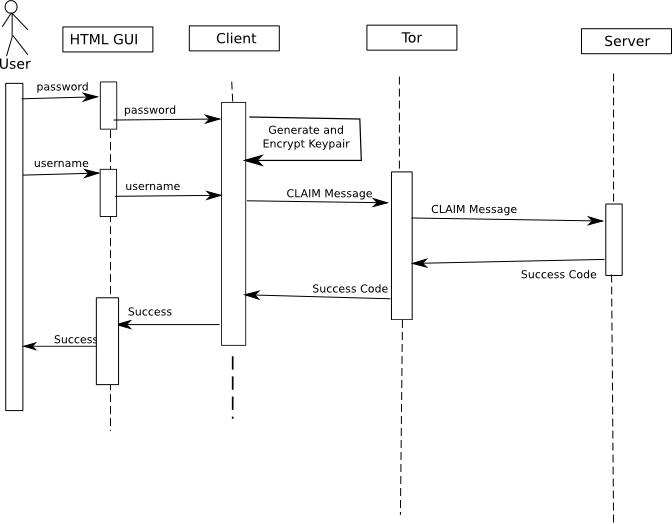
\includegraphics[width=\textwidth]{images/design/sequence_first.png}
    \caption{Sequence Diagram - Registering}
    \label{fig:sequencef}
\end{figure}

\begin{figure}[h]
    \centering
    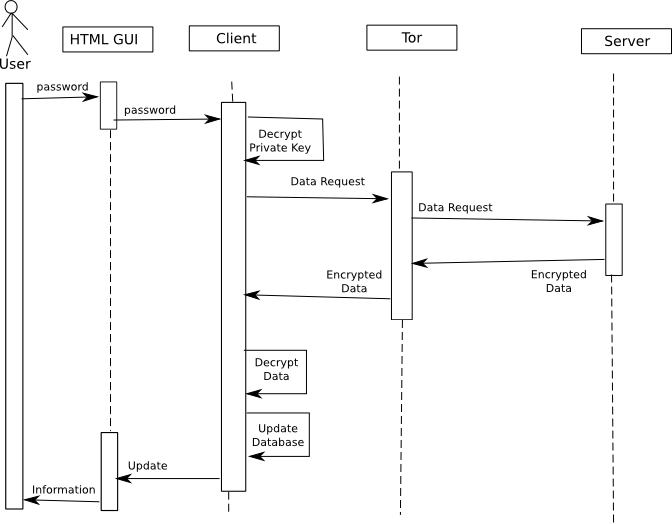
\includegraphics[width=\textwidth]{images/design/sequence_recieve.png}
    \caption{Sequence Diagram - Recieving Data}
    \label{fig:sequencer}
\end{figure}

\begin{figure}[h]
    \centering
    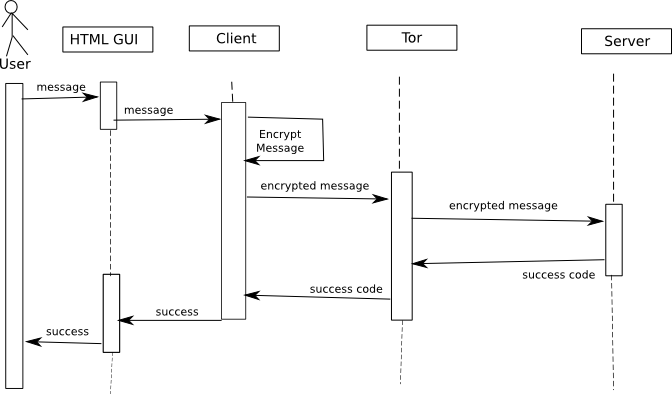
\includegraphics[width=\textwidth]{images/design/sequence_send.png}
    \caption{Sequence Diagram - Sending Data}
    \label{fig:sequences}
\end{figure}
